\section{Esgrima}

La esgrima es un deporte de estrategia en el cuál tendrás que analizar a tu
 oponente a la vez que te defiendes de sus acometidas. Al mismo tiempo, tendrás que
 disfrazar tus ataques con otros para que el oponente no sea capaz de analizar
 tus movimientos. Es por esto por lo que la mayoría de practicantes lo denominan
 el ajedrez en movimiento puesto que todo son ataques, por un franco u otro,
 pequeñas batallas que te llevarán a ganar la guerra al final. Jugar con la mente
 del rival y calmar la tuya para tener superioridad táctica.

Por supuesto que el físico influye en este deporte, no deja de ser un deporte de contacto
 en el cual las cualidades físicas (fuerza, agilidad, rapidez, coordinación, reflejos, etc)
 son un factor mas a tener en cuenta, pero esto no serán mas que componentes de una ecuación
 la cual nos dará la victoria.

Ahora pasaremos a explicar por encima en que consiste un asalto de esgrima.
 Un asalto de esgrima es un enfrentamiento entre dos
 oponentes los cuales tienen que llegar al límite de tocados antes que el rival o haber obtenido mayor puntuación
 una vez haya terminado el tiempo de asalto. Dependiendo de la modalidad y categoría
 variaran estos tiempos y límite de tocados. ¿Pero que es un tocado? Un tocado no es mas que
 un punto a tu favor, el cual se puede conseguir tocando al rival o mediante sanciones del rival.
 Un ejemplo de sanciones podría ser un comportamiento antideportivo, salirse de la pista por el fondo,
 dar varias veces la espalda, perder el tiempo repetidas veces mientras vas perdiendo, etc.

Como la mayoría de artes marciales no es mas que un esquema táctico en el cuál tendremos unas variables
 de entrada mediante las cuales determinaremos una salida. ¿Pero como es posible que un deporte de contacto
 se base en una serie de entradas y salidas? Bien, un ejemplo muy básico es el siguiente: ante una acción ofensiva
 directa hacia la parte superior del cuerpo lo lógico es cubrirse esta parte. Aquí es donde entra en juego
 la estrategia de cada componente del combate. Si el atacante sabe que tu reacción ante una amenaza arriba
 será cubrirte esa zona, el amagará con un ataque falso (finta) a una parte del cuerpo y sobre tu acción
 defensiva para evitar esta acometida aprovechará para atacar otra zona que dejaste descubierta por
 defender la primera acción. Por otro lado, el defensor puede analizar al rival y saber que el primer ataque
 no será el verdadero, si no que será una preparación para atacar sobre otra zona, de este modo anticiparse
 y atacar sobre esta preparación o amagar con defenderse sobre la primera zona para después cubrirse la segunda
 y contra-atacar.

\subsection{Modalidad de espada en esgrima}

Una vez tenemos unas nociones básicas sobre como funciona un esquema táctico en general sobre cualquier
 disciplina de arte marcial o deporte de contacto, pasemos a hablar de la esgrima en concreto.
 Hay tres disciplinas dentro de este deporte: sable, florete y espada. Siendo la primera una modalidad
 en la que se puede tocar con cualquier parte de la hoja, mientras que en las dos últimas son armas de
 estoque, es decir, solo vale tocar con la punta. Puesto que cada modalidad tiene unas normas y la espada
 es la mas practicada y mas sencilla de todas, nos centraremos en ella. En la modalidad de espada se puede
 tocar en cualquier parte del cuerpo, esto incluye desde el pecho, hasta la suela de la zapatilla, pasando
 por la espalda o cualquier lugar que se nos ocurra. Con la única excepción de la nuca, puesto que es la única
 zona en la que no hay protección, para ello hay normas evitando que des la espalda y expongas esta zona
 tan delicada.

% https://es.m.wikipedia.org/wiki/Archivo:Fencing_epee_valid_surfaces.svg
\begin{figure}[htb]
	\centering
	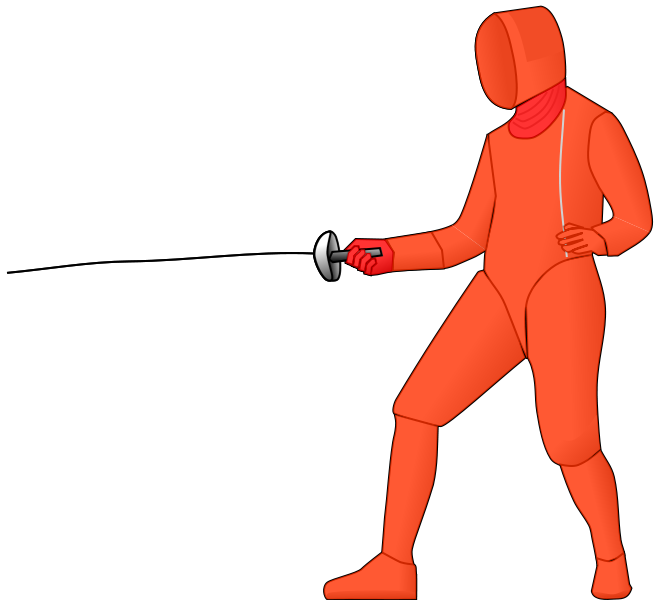
\includegraphics[width=0.4\linewidth]{blancoValido}
	\caption[Blanco válido espada]{Blanco válido espada}
	\label{fig:blancoValido}
\end{figure}

Como hemos mencionado antes es un arma de estoque, por lo que el mecanismo de activación estará en la punta
 y será mediante un botón, el cuál al presionarse sobre un blanco válido cerrará un circuito electrico cuyo
 objetivo es señalizar el tocado. A partir de este momento el rival tiene un breve periodo de tiempo, 0.4 segundos,
 para realizar un tocado sobre el rival y que haya un tocado doble. Pasado este tiempo el circuito se bloqueará
 y solo será efectivo el primer tocado. A pesar de que haya un tocado doble no quiere decir que siempre sean válidos
 ambos tocados. Mediante las normas se dictaminará si los dos lo son, solo uno o ninguno de ellos lo es.
 Un ejemplo podría ser que uno de los dos tiradores se encuentre fuera de la pista, lo cual anularía su tocado.
 Como se han podido dar cuenta, hemos hablado de tiempo, por lo que otro componente a tener en cuenta es ser mas
 rápido que el rival, esto habrá que tenerlo en cuenta en nuestro esquema táctico para poder decidir una acción en
 la cual, aunque nos toquen, nosotros lo hagamos con suficiente antelación al rival de modo que su tocado no
 sea válido.

Tal y como se habló antes los asaltos tienen un límite de tiempo y un límite de tocados,
 este será otro factor a tener en cuenta en nuestro esquema táctico sobre como plantear el asalto.
 Puede que a veces nos interese llevar un asalto hasta el final del tiempo desgastando físicamente al
 rival para aprovechar esta superioridad al final. Otras veces quizás nos interese lo contrario,
 acabar con el asalto cuanto antes para evitar dejar al contrario pensar. Puede que otras veces nos
 interese alargar el asalto al mayor número de tocados posibles puesto que tengamos mayor
 repertorio que nuestro oponente, mientras que en el caso contrario, si tenemos pocas acciones nos interesará
 hacer el menor número de tocados. También habrá que tener en cuenta el marcador y cuanta ventana hay
 hasta el final del combate, si al rival le falta un tocado para ganar, mientras que a nosotros nos faltan
 tres, no nos interesa que haya un tocado doble puesto que el ganaría. Estas son algunas de las variables
 entran dentro de la formula para plantear nuestra táctica en un asalto de esgrima.

\subsection{Estructura competición esgrima}

Una vez que ya sabemos como funciona un asalto de esgrima podemos hablar sobre como funciona una competición
 de esgrima. Primero hablaremos de las individuales y mas tarde de los equipos. Se explicará el funcionamiento
 de una competición estandar, lo cual puede variar en función de la categoría y tipo de competición, puesto que
 existen varios formatos para las competiciones amistosas.
 En cuanto a las competiciones individuales primero se disputa una fase de grupos, la cual se denomina
 \textit{poule} en la cual se dividen a todos los tiradores en poules (grupos) de seis o siete tiradores en función
 del número de participantes que haya. Siendo siete el número ideal y dejando las de seis en caso de que
 no haya número suficiente de tiradores. Estas poules se hacen en función del ranking de los tiradores inscritos
 a la competición, de manera que estén lo mas equilibradas posibles. A destacar que hay un sistema para realizarlas y no
 es a intuición del directorio. Una vez organizadas los poules se da
 comienzo a ellas. En ellas se enfrentan todos los tiradores entre ellos, empezando los que sean del mismo
 país y club, para evitar favoritismos mas adelante. Estos enfrentamientos serán en un único asalto con un
 límite de cinco tocados y una duración máxima de tres minutos. El primero que llegue al límite con diferencia
 de un tocado o quien tenga mayor puntuación al acabar el tiempo será el ganador de este encuentro. El orden
 de enfrentamiento entre tiradores también está pre-establecido según la posición dentro de la poule.
 En los anexos se podrá encontrar una ejemplo de hoja de poule.

\begin{table}[htb]%
  \centering
  \caption{Ejemplo tabla resultados poule}
  \label{tab:anchura}
  \begin{tabular}{ | l | l | l | l | l | l | l | l | }
    \hline
    & Tirador 1 & Tirador 2 & Tirador 3 & Tirador 4 & Tirador 5 & Tirador 6 & Tirador 7 \\ \hline
    Tirador 1 & x & V & & & & & \\ \hline
    Tirador 2 & 1 & x & & & & & \\ \hline
    Tirador 3 & & & x & & & & \\ \hline
    Tirador 4 & & & & x & & & 2 \\ \hline
    Tirador 5 & & & & & x & & \\ \hline
    Tirador 6 & & & & & & x & \\ \hline
    Tirador 7 & & & & $V_3$ & & & x \\
    \hline
  \end{tabular}
\end{table}

La anterior tabla sería un ejemplo de una tabla de poule en mitad de una competición. Se puede apreciar como se anotan
 las victorias, las derrotas y los resultados de ambas. En caso de obtener una victoria se anotará la puntuación. Una vez
 terminadas todas las poules se obtendrá la clasificación general, obteniendose de la siguiente manera:

\begin{compactenum}
  \item Porcentaje Victorias/Derrotas
  \item Tocados dados - Tocados recibidos
  \item Tocados dados
\end{compactenum}

%En caso de empate de todo lo anterior ambos mantendrán el mismo número de serie y se saltará el siguiente. El orden de
% quien estará encima de otro será aleatorio. Una vez obtenida la clasificación general de las poules, se hace un corte
% para eliminar a un porcentaje de los participantes, suele ser un veinte por ciento. Con los tiradores restantes
% de este corte se hace un tablón lo suficientemente grande para acoger a todos los participantes. El número de este
% tablón será una potencia de dos, es decir 2, 4, 8, 16, 32, 64, etc. En caso de no haber participantes suficientes para completar
% el tablón los primeros participantes pasarán exentos de la primera ronda. El resto de la competición es una eliminatoria
% directa en la que el vencedor pasa a la siguiente ronda mientras que el perdedor termina la competición.

Debido a que cada punto cuenta desde el inicio, ya que esto determinará como de fácil será el camino en la competición
todas y cada una de las decisiones que tomemos deberán ser lo mas óptimas posibles. Para ello muchas veces contamos
con nuestra experiencia, entrenadores o incluso compañeros que nos ayudarán a tomar una decisión dandonos su opinión.
Pero como no siempre será este el caso, se quiere desarrollar una herramienta la cual nos facilite la toma de
decisiones en mitad de la competición. Para ello usaremos un sistema de apoyo a la decisión, a partir de ahora
lo denominaremos como DSS (del inglés Decision Support System).
